\documentclass[a4paper, 14pt]{article}
\usepackage[margin=1.6cm]{geometry}
\usepackage[utf8]{inputenc}
\usepackage{minted}
\usepackage[russian]{babel}
\usepackage{amsmath}
\usepackage{graphicx}
\usepackage{changepage}
\usepackage{hyperref}
\usepackage{cases}
\usepackage{tikz-timing}[2017/12/20]
\usepackage{relsize}
\usepackage{booktabs}
\usepackage{gensymb}
\usepackage{multirow}
\usepackage{longtable}
\usetikzlibrary {arrows.meta}

\hypersetup{
	linkbordercolor = {1 1 1}
}

\usepackage{tikz-timing}[2009/05/15]
\usepackage{multicol}
\usepackage[T2A]{fontenc}
\usepackage{pgfplots}
%\usepackage[left=2.5cm, right=1.5cm, vmargin=2.5cm]{geometry}
\setlength\parindent{0pt} % Удалить отступы из параграфов.

\usepackage{listings}
\usepackage{caption}
\DeclareCaptionFont{white}{\color{white}} % Текст заголовка.
\DeclareCaptionFormat{listing}{\colorbox{gray}{\parbox{\textwidth}{#1#2#3}}}
\captionsetup[lstlisting]{format=listing,labelfont=white,textfont=white}
\renewcommand\labelenumi{\theenumi)}
\setlength\parindent{24pt}



\begin{document}
\lstset{
    language=java,                 % Выбор языка для подсветки (здесь это java).
    basicstyle=\small\sffamily,    % Размер и начертание шрифта для подсветки кода.
    numbers=left,                  % Где поставить нумерацию строк (слева\справа).
    numberstyle=\tiny,             % Размер шрифта для номеров строк.
    stepnumber=1,                  % Размер шага между двумя номерами строк.
    firstnumber=1,
    numberfirstline=true
    numbersep=5pt,                 % Как далеко отстоят номера строк от подсвечиваемого кода.
    backgroundcolor=\color{white}, % Цвет фона подсветки - используем \usepackage{color}.
    showspaces=false,              % Показывать или нет пробелы специальными отступами.
    showstringspaces=false,        % Показывать или нет пробелы в строках.
    showtabs=false,                % Показывать или нет табуляцию в строках.
    frame=single,                  % Рисовать рамку вокруг кода.
    tabsize=2,                     % Размер табуляции по умолчанию равен 2 пробелам.
    captionpos=t,                  % Позиция заголовка вверху [t] или внизу [b].
    breaklines=true,               % Автоматически переносить строки (да\нет).
    breakatwhitespace=false,       % Переносить строки только если есть пробел.
    escapeinside={\%*}{*)}         % Если нужно добавить комментарии в коде.
}

\begin{titlepage}
    \center

    ФЕДЕРАЛЬНОЕ ГОСУДАРСТВЕННОЕ АВТОНОМНОЕ ОБРАЗОВАТЕЛЬНОЕ УЧРЕЖДЕНИЕ ВЫСШЕГО ОБРАЗОВАНИЯ\linebreak
    «Санкт-Петербургский политехнический университет Петра Великого»
    \noindent\rule{500pt}{0.8pt} \\
    \textsc{\Large Институт компьютерных наук и кибербезопасности}\\
    \textsc{\large Высшая школа программной инженерии}\\[1.5cm]

    { \huge \bfseries ОТЧЕТ ПО ИНТЕГРАЦИОННОМУ ТЕСТИРОВАНИЮ	\\
    \Large \mdseries АГРЕГАТОР ЦИФРОВЫХ ФИНАНСОВЫХ АКТИВОВ <<ТЕССЕРАКТ>> \\
    \large по дисциплине <<Технологии разработки качественного программного обеспечения>>}\\
    \flushright{
        {\phantom{qwe}}\\[1.0cm]
    }

    \begin{figure}[H]
        \centering
        
\includegraphics[width=10cm]{./resources/1.png}\\[2.0cm]
    \end{figure}

    \begin{multicols}{2}
        \begin{flushright} \large

            {Выполнили студенты группы: 5130904/00104:}\\
            {\phantom{qwe}}\\
            {\phantom{qwe}}\\
            {\phantom{qwe}}\\
            {\phantom{qwe}}\\

            {Преподаватель:\\}

        \end{flushright}
        \begin{flushright}

            {Почернин В. С.}\\
            {Шиляев В. С.}\\
            {Мурзаканов И. М.}\\
            {Разукрантов В. Е.}\\[0.5cm]


            Маслаков А. П.\\

        \end{flushright}
    \end{multicols}

    \flushright{
        {\phantom{qwe}}\\[0.5cm]
    }
    \centering{
        Санкт-Петербург\\
        2024
    }

    \vfill
\end{titlepage}

\Large
\tableofcontents
\newpage
\large

\section{Постановка задачи}

Интеграционное тестирование предполагает наличие нескольких модулей или, если приложение построено в соответствии с микросервисной архитектурой, микросервисов разработанного приложения. В качестве модулей могут быть функциональные части (например: модуль авторизации/аутентификации, модуль взаимодействия с пользователем, модуль интеграции со сторонним сервисом).

Необходимо выполнить интеграционное тестирование нескольких модулей в соответствии с предварительно описанными сценариями тестирования. Каждый сценарий тестирования должен представлять собой некоторый законченный вариант использования системы (кейс) пользователя.

Интеграционное тестирование предполагает командную работу над программным продуктом, поэтому необходимо проводить его с использованием одного из инструментов \texttt{CI}, доступных на рынке: \texttt{Gitlab}, \texttt{Jenkins}, \texttt{Bamboo}, \texttt{TeamCity}, etc.

Минимальное количество сценариев - 10.

\subsection{Обязательные требования}

\begin{enumerate}
    \item Предварительное формирование документа, описывающего тестовые сценарии.
    \item Применение заглушек (mock-сервисов или mock-объектов) для изоляции от окружения и внешних сервисов или для ускорения прохождения тестов.
    \item Рассмотрение негативных сценариев тестирования.
    \item Поднятие сервера непрерывной интеграции и запуск задачи по интеграционному тестированию по временному триггеру или по событию изменения кода приложения/интеграционных тестов.
\end{enumerate}

\subsection{Содержание отчета}

Отчет по интеграционному тестированию должен содержать:

\begin{enumerate}
    \item Отчет о выполненной работе, использованных инструментах, примененных техниках тест-дизайна.
    \item Тест-план со словесным описанием тестовых сценариев, которые планируется реализовать в интеграционном тестировании.
    \item Отчет о прохождении тестов с результатами на сервере непрерывной интеграции.
    \item Описание процедуры расширения тестового набора на примере добавления новой функциональной части (или модуля).
\end{enumerate}

\section{Ход работы}

\subsection{Отчет о выполненной работе, использованных инструментах, примененных техниках тест-дизайна}

В рамках проведенной работы, код серверной части приложения был покрыт интеграционными тестами.

\subsubsection{Использованные инструменты}

Были использованы следующие инструменты:

\begin{itemize}
    \item \texttt{JUnit} - фреймворк для языков программирования \texttt{Java} и \texttt{Kotlin}, предназначенный для автоматического unit-тестирования. Данный фреймворк позволяет удобно создавать, организовывать и выполнять тесты, благодаря широкому набору аннотаций и встроенной поддержки в популярных IDE. Для серверной части применялся \texttt{JUnit5}.
    \item \texttt{Spring Boot Test} - предоставляет инструменты для интеграционного тестирования \texttt{Spring Boot} приложений, включая поддержку тестирования в изолированном контексте приложения.
    \item \texttt{MockMvc} - инструмент из \texttt{Spring Test} для тестирования контроллеров в изоляции от сервлет контейнера. Позволяет отправлять \texttt{HTTP} запросы и проверять ответы без запуска сервера.
    \item \texttt{Testcontainers} - библиотека, которая поддерживает тесты, использующие \texttt{Docker} контейнеры. В нашем случае использовалась для поднятия \texttt{PostgreSQL} базы данных в \texttt{Docker} для тестирования взаимодействия с БД.
    \item \texttt{Flyway} - инструмент для версионирования базы данных, который применялся для миграции схемы и данных БД перед выполнением тестов.
    \item \texttt{GitHub Actions} - система непрерывной интеграции (\texttt{CI}), используемая нами для автоматического выполнения тестов при открытии \texttt{PR} или мерже в мастер ветку. Позволяет автоматизировать процесс интеграционного тестирования и не только.
\end{itemize}

\subsubsection{Примененные техники тест-дизайна}

\textbf{Тест-дизайн} - это процесс разработки техник и методов тестирования. Главная задача тест-дизайна - разработать сценарии, которые позволяют протестировать максимальное количество функций за минимальное время. Таким образом, разрабатывается тестовая документация, опирающаяся на общие принципы и логику тестирования с поправкой на особенности продукта. Суть всех техник тест-дизайна - оптимизировать процесс тестирования.

Нами были применены следующие техники тест-дизайна:

\begin{itemize}
    \item \textbf{Классы эквивалентности}: данная техника тестирования состоит в том, что все тестовые кейсы группируются и разделяются на некие эквивалентные классы. При этом классы одной тестовой группы ведут себя одинаково. То есть, если система корректно обработает одно значение из класса, то она корректно обработает и все остальные значения из этого класса. Согласно одному из принципов тестирования - <<полное тестирование программы невозможно, или займет недопустимо длительное время, поскольку в этом случае необходимо проверять слишком много комбинаций тестовых данных>>.

    Данная техника позволяет получить четкие результаты за ограниченное время, улучшает качество тест-кейсов, устраняя избыточность, при этом покрывая тестовые сценарии.

    Приведем пример теста:
    \normalsize
    \inputminted[frame=single]{java}{./code/2.java}
    \large

    В данном примере тестируется корректность регистрации при вводе некорректного пароля. Вместо того, чтобы тестировать всевозможные комбинации паролей, мы разбиваем их на классы эквивалентности, такие как:
    \begin{itemize}
        \item Пустой пароль;
        \item Слишком короткий пароль;
        \item Слишком длинный пароль;
        \item Пароль без букв;
        \item Пароль без цифр или специальных символов;
        \item Пароль с некорректными символами;
    \end{itemize}

    \item \textbf{Граничные условия}: при использовании данной техники тестирования, основное внимание уделяется значениям на границах допустимого диапазона, поскольку зачастую ошибки возникают именно в граничных точках - такая проверка помогает их быстро находить.

    Граничные значения - это такие места, в которых один класс эквивалентности переходит в другой. Это значения на границе допустимого диапазона входных данных, которые могут привести к изменению поведения программы.

    При использовании данной техники на каждой границе диапазона следует проверить по три значения:
    \begin{itemize}
        \item Граничное значение;
        \item Значение перед границей;
        \item Значение после границы;
    \end{itemize}

    Приведем пример теста:
    \small
    \inputminted[frame=single]{java}{./code/3.java}
    \large

    Для создания диверсификаций у нас работает следующая логика: сумма диверсификации не должна быть меньше, чем стоимость самого дешевого актива и не должна быть больше, чем определенная граница (10 миллионов рублей). Уровень рискованности, в свою очередь, может принимать значения 0, 1, 2 или 3.

    Таким образом, мы проверяем правильность работы алгоритма на границах диапазонов.

    \item \textbf{Попарное тестирование}: эта методика тестирования, при которой создаются тестовые случаи для проверки комбинаций каждой пары входных параметров. Это помогает значительно сократить количество тестов при сохранении высокого уровня покрытия, поскольку исследования показывают, что большинство ошибок вызывается взаимодействием между парой параметров.

    Приведем пример теста:
    \normalsize
    \inputminted[frame=single]{java}{./code/4.java}
    \large

    Мы тестируем метод, который проверяет корректность трех полей - логина, адреса электронной почты и пароля. Если брать полную таблицу состояний - мы будем должны написать 8 тестов:

    \begin{table}[H]
        \centering
        \begin{tabular}{|c|c|c|c|}
        \hline
        \textbf{}  & \textbf{login} & \textbf{email} & \textbf{password} \\ \hline
        \textbf{1} & valid          & valid          & valid             \\ \hline
        \textbf{2} & valid          & valid          & invalid           \\ \hline
        \textbf{3} & valid          & invalid        & valid             \\ \hline
        \textbf{4} & valid          & invalid        & invalid           \\ \hline
        \textbf{5} & invalid        & valid          & valid             \\ \hline
        \textbf{6} & invalid        & valid          & invalid           \\ \hline
        \textbf{7} & invalid        & invalid        & valid             \\ \hline
        \textbf{8} & invalid        & invalid        & invalid           \\ \hline
        \end{tabular}
    \end{table}

    Однако, используя технику попарного тестирования, мы можем сократить количество тестов до 4-х:
    \begin{table}[H]
        \centering
        \begin{tabular}{|c|c|c|c|}
        \hline
        \textbf{}  & \textbf{login} & \textbf{email} & \textbf{password} \\ \hline
        \textbf{1} & valid          & valid          & valid             \\ \hline
        \textbf{2} & valid          & invalid        & invalid           \\ \hline
        \textbf{3} & invalid        & invalid        & valid             \\ \hline
        \textbf{4} & invalid        & valid          & invalid           \\ \hline
        \end{tabular}
    \end{table}
\end{itemize}

\subsection{Тест-план со словесным описанием тестовых сценариев которые были реализованы в интеграционном тестировании}

Описание тест-плана удобно разделить на классы, созданные для тестирования.

\subsubsection{AssetControllerTest.java}

Данный класс тестирует контроллер активов.

\begin{enumerate}
    \item \texttt{givenPageNumber\_whenGetAssets\_thenReturnsAssetsWithExpectedIds} - получение первых 10 и вторых 10 активов (имитация постраничной загрузки).
    \item \texttt{givenAssetId10\_whenGetAsset\_thenReturnsExpectedAsset} - получение конкретного актива.
    \item \texttt{givenNonExistent\_whenGetAsset\_thenReturnsExpectedError} - получение несуществующего актива.
\end{enumerate}

\subsubsection{AuthenticationControllerTest.java}

Данный класс тестирует контроллер аутентификации.

\begin{enumerate}
    \item \texttt{givenValidCredentials\_whenRegister\_thenSuccess} - регистрация с корректными данными.
    \item \texttt{givenInvalidRegisterRequest\_whenRegister\_thenBadRequest} - регистрация с некорректными данными.
    \item \texttt{givenCredentialsWithExistingLogin\_whenRegister\_thenReturnsExpectedError} - регистрация, когда пользователь уже существует.
    \item \texttt{givenCredentialsWithExistingEmail\_whenRegister\_thenReturnsExpectedError} - регистрация, когда email уже существует.
    \item \texttt{givenInvalidLogin\_whenRegister\_thenReturnsExpectedError} - регистрация с некорректным логином.
    \item \texttt{givenInvalidPassword\_whenRegister\_thenReturnsExpectedError} - регистрация с некорректным паролем.
    \item \texttt{givenInvalidEmail\_whenRegister\_thenReturnsExpectedError} - регистрация с некорректным email.
    \item \texttt{givenCorrectCredentials\_whenLogin\_thenReturnsToken} - аутентификация с корректными данными.
    \item \texttt{givenNonExistentLogin\_whenLogin\_thenReturnsExpectedError} - аутентификация с несуществующим логином.
    \item \texttt{givenNonExistentPassword\_whenLogin\_thenReturnsExpectedError} - аутентификация с несуществующим паролем.
    \item \texttt{givenCorrectRequest\_whenChangePassword\_thenSuccess} - корректное изменение пароля.
    \item \texttt{givenNonExistentOldPassword\_whenChangePassword\_thenReturnsExpectedError} - изменение пароля, когда старый пароль не совпадает с тем, что лежит в базе.
    \item \texttt{givenIncorrectNewPassword\_whenChangePassword\_thenReturnsExpectedError} - изменение пароля, когда пароль некорректный.
\end{enumerate}

\subsubsection{DiversificationControllerTest.java}

Данный класс тестирует контроллер диверсификаций.

\begin{enumerate}
    \item \texttt{givenCorrectRequest\_whenGetDiversifications\_thenReturnsDiversificationsWithExpectedIds} - получить первые 10 своих диверсификаций.
    \item \texttt{givenDiversificationId2\_whenGetDiversification\_thenReturnsExpectedDiversification} - получить свою существующую диверсификацию.
    \item \texttt{givenNonExistentOrNonYourDiversification\_whenGetDiversification\_thenReturnsExpectedError} - получить не свою или несуществующую диверсификацию.
    \item \texttt{givenValidCreateDiversificationRequest\_whenCreateDiversification\_thenSuccess} - создание диверсификации с корректными данными.
    \item \texttt{givenInvalidCreateDiversificationRequest\_whenCreateDiversification\_thenReturnsExpectedError} - создание диверсификации с некорректными данными.
\end{enumerate}

\subsubsection{FavouritesControllerTest.java}

Данный класс тестирует контроллер избранного.

\begin{enumerate}
    \item \texttt{givenCorrectRequest\_whenGetFavourites\_thenReturnsFavouritesWithExpectedIdsAndStatus} - получить первые 10 своих избранных активов.
    \item \texttt{givenExistsAssetId\_whenAddFavourites\_thenSuccess} - добавить существующий актив в избранное.
    \item \texttt{givenExistsAssetId\_whenRemoveFavourites\_thenSuccess} - удалить существующий актив из избранного.
    \item \texttt{givenNonExistentAssetId\_whenAddFavourites\_thenSuccess} - добавить несуществующий актив в избранное.
    \item \texttt{givenNonExistentAssetId\_whenRemoveFavourites\_thenSuccess} - удалить несуществующий актив из избранного.
\end{enumerate}

\subsubsection{BadRequestTest.java}

Данный класс тестирует некорректные тела запросов.

\begin{enumerate}
    \item \texttt{givenInvalidQueryParams\_whenHandleGetRequest\_thenReturnsExpectedError} - некорректные query параметры GET запроса.
    \item \texttt{givenIncorrectPathParams\_whenHandleGetRequest\_thenReturnsExpectedError} - некорректные параметры пути GET запроса.
    \item \texttt{givenIncorrectPathParams\_whenHandlePostRequest\_thenReturnsExpectedError} - некорректные параметры пути POST запроса.
    \item \texttt{givenIncorrectPathParams\_whenHandleDeleteRequest\_thenReturnsExpectedError} - некорректные параметры пути DELETE запроса.
    \item \texttt{givenIncorrectBodyParams\_whenHandlePostRequest\_thenReturnsExpectedError} - некорректные параметры тела POST запроса.
    \item \texttt{givenIncorrectBodyParams\_whenHandlePutRequest\_thenReturnsExpectedError} - некорректные параметры тела PUT запроса.
\end{enumerate}

\subsubsection{UnauthorizedTest.java}

Данный класс тестирует некорректный токен аутентификации.

\begin{enumerate}
    \item \texttt{givenBadCredentials\_whenHandleGetRequest\_thenReturnsExpectedError} - некорректные параметры аутентификации GET запроса.
    \item \texttt{givenBadCredentials\_whenHandlePostRequest\_thenReturnsExpectedError} - некорректные параметры аутентификации POST запроса.
    \item \texttt{givenBadCredentials\_whenHandlePutRequest\_thenReturnsExpectedError} - некорректные параметры аутентификации PUT запроса.
    \item \texttt{givenBadCredentials\_whenHandleDeleteRequest\_thenReturnsExpectedError} - некорректные параметры аутентификации DELETE запроса.
\end{enumerate}

\subsection{Отчет о прохождении тестов с результатами на сервере непрерывной интеграции}

За работу сервера непрерывной интеграции отвечает конфигурационный файл \texttt{integration\_tests.yml}:
\small
\inputminted[frame=single]{yaml}{./code/1.yml}
\large

Как можно заметить, мы выполняем следующие шаги:

\begin{itemize}
    \item Копируем наш репозиторий в систему непрерывной интеграции.
    \item Устанавливаем виртуальную машину \texttt{Java}.
    \item Устанавливаем \texttt{Gradle}.
    \item Запускаем тесты с помощью \texttt{Gradle}.
    \item Загружаем артефакты тестов в систему интеграции.
\end{itemize}

Как можно заметить, запуск данного сценария происходит при следующих условиях:

\begin{itemize}
    \item Произошел пуш в мастер-ветку.
    \item Открылся \texttt{PR} в мастер-ветку.
\end{itemize}

Страница с пройденным \texttt{CI} выглядит следующим образом:

\begin{figure}[H]
    \centering
    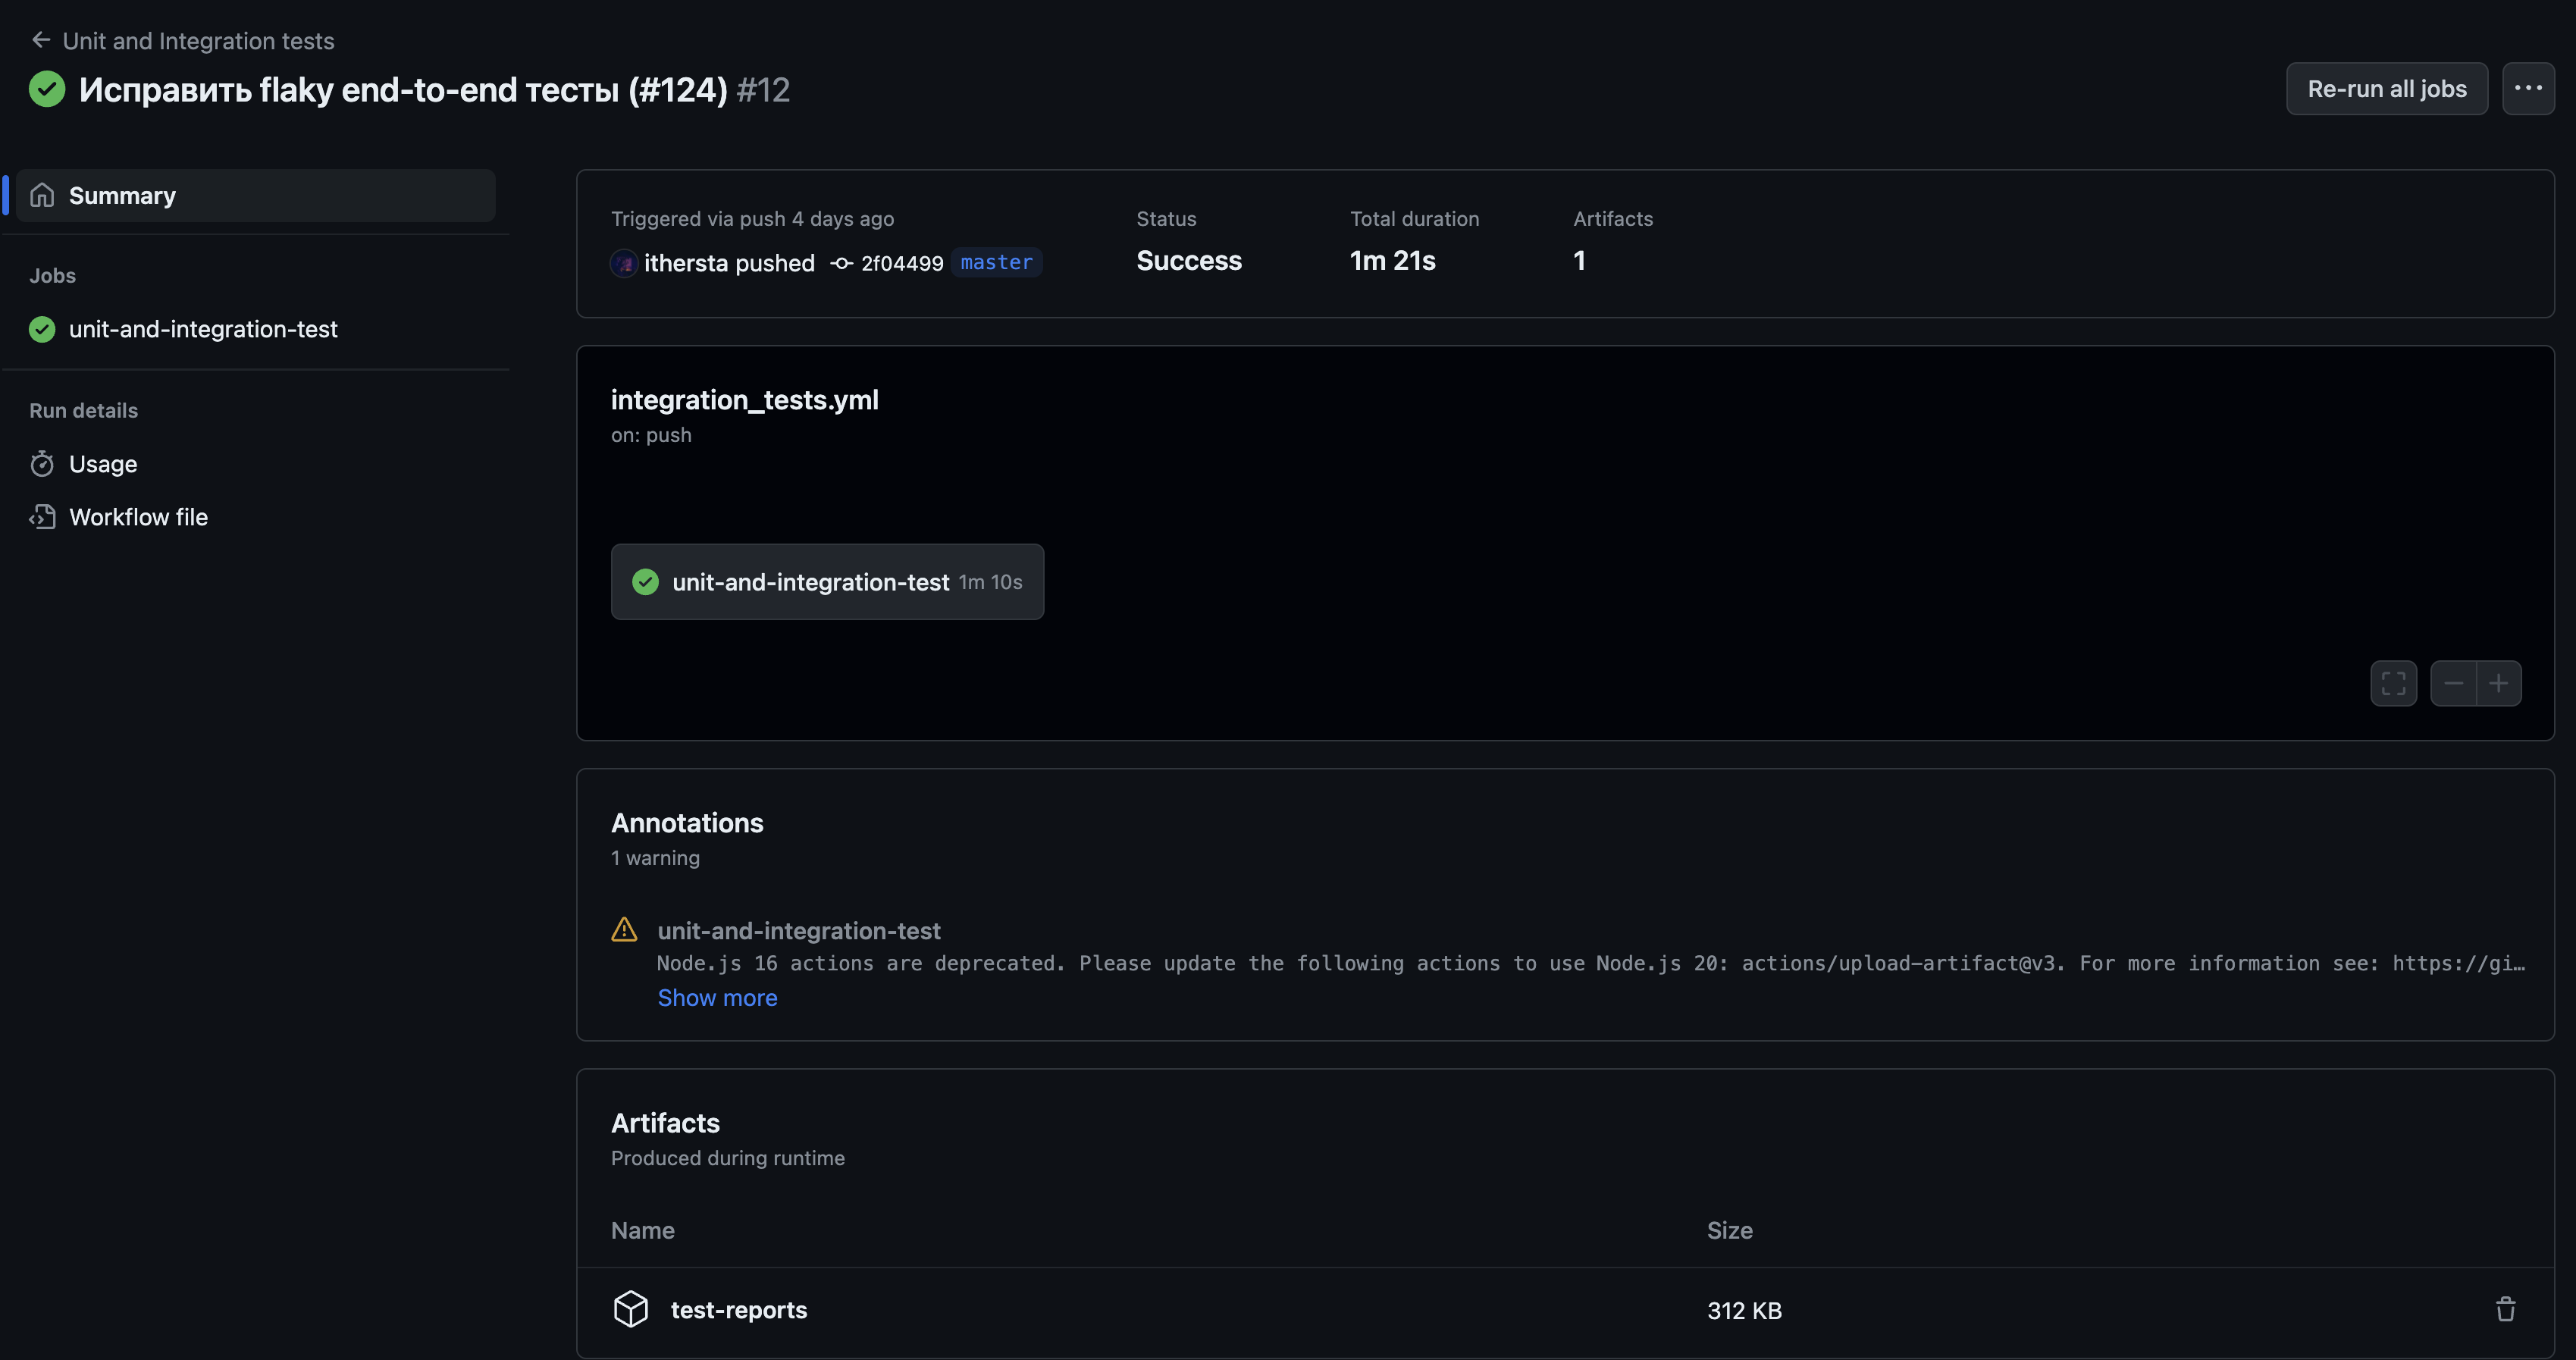
\includegraphics[width=17cm]{resources/2.png}\\
    \caption{Пройденный \texttt{CI}}
\end{figure}

Ниже можно скачать архив с артефактами тестирования. Он содержит в себе \texttt{HTML}-страницу с подробным отчетом о пройденных тестах.

\begin{figure}[H]
    \centering
    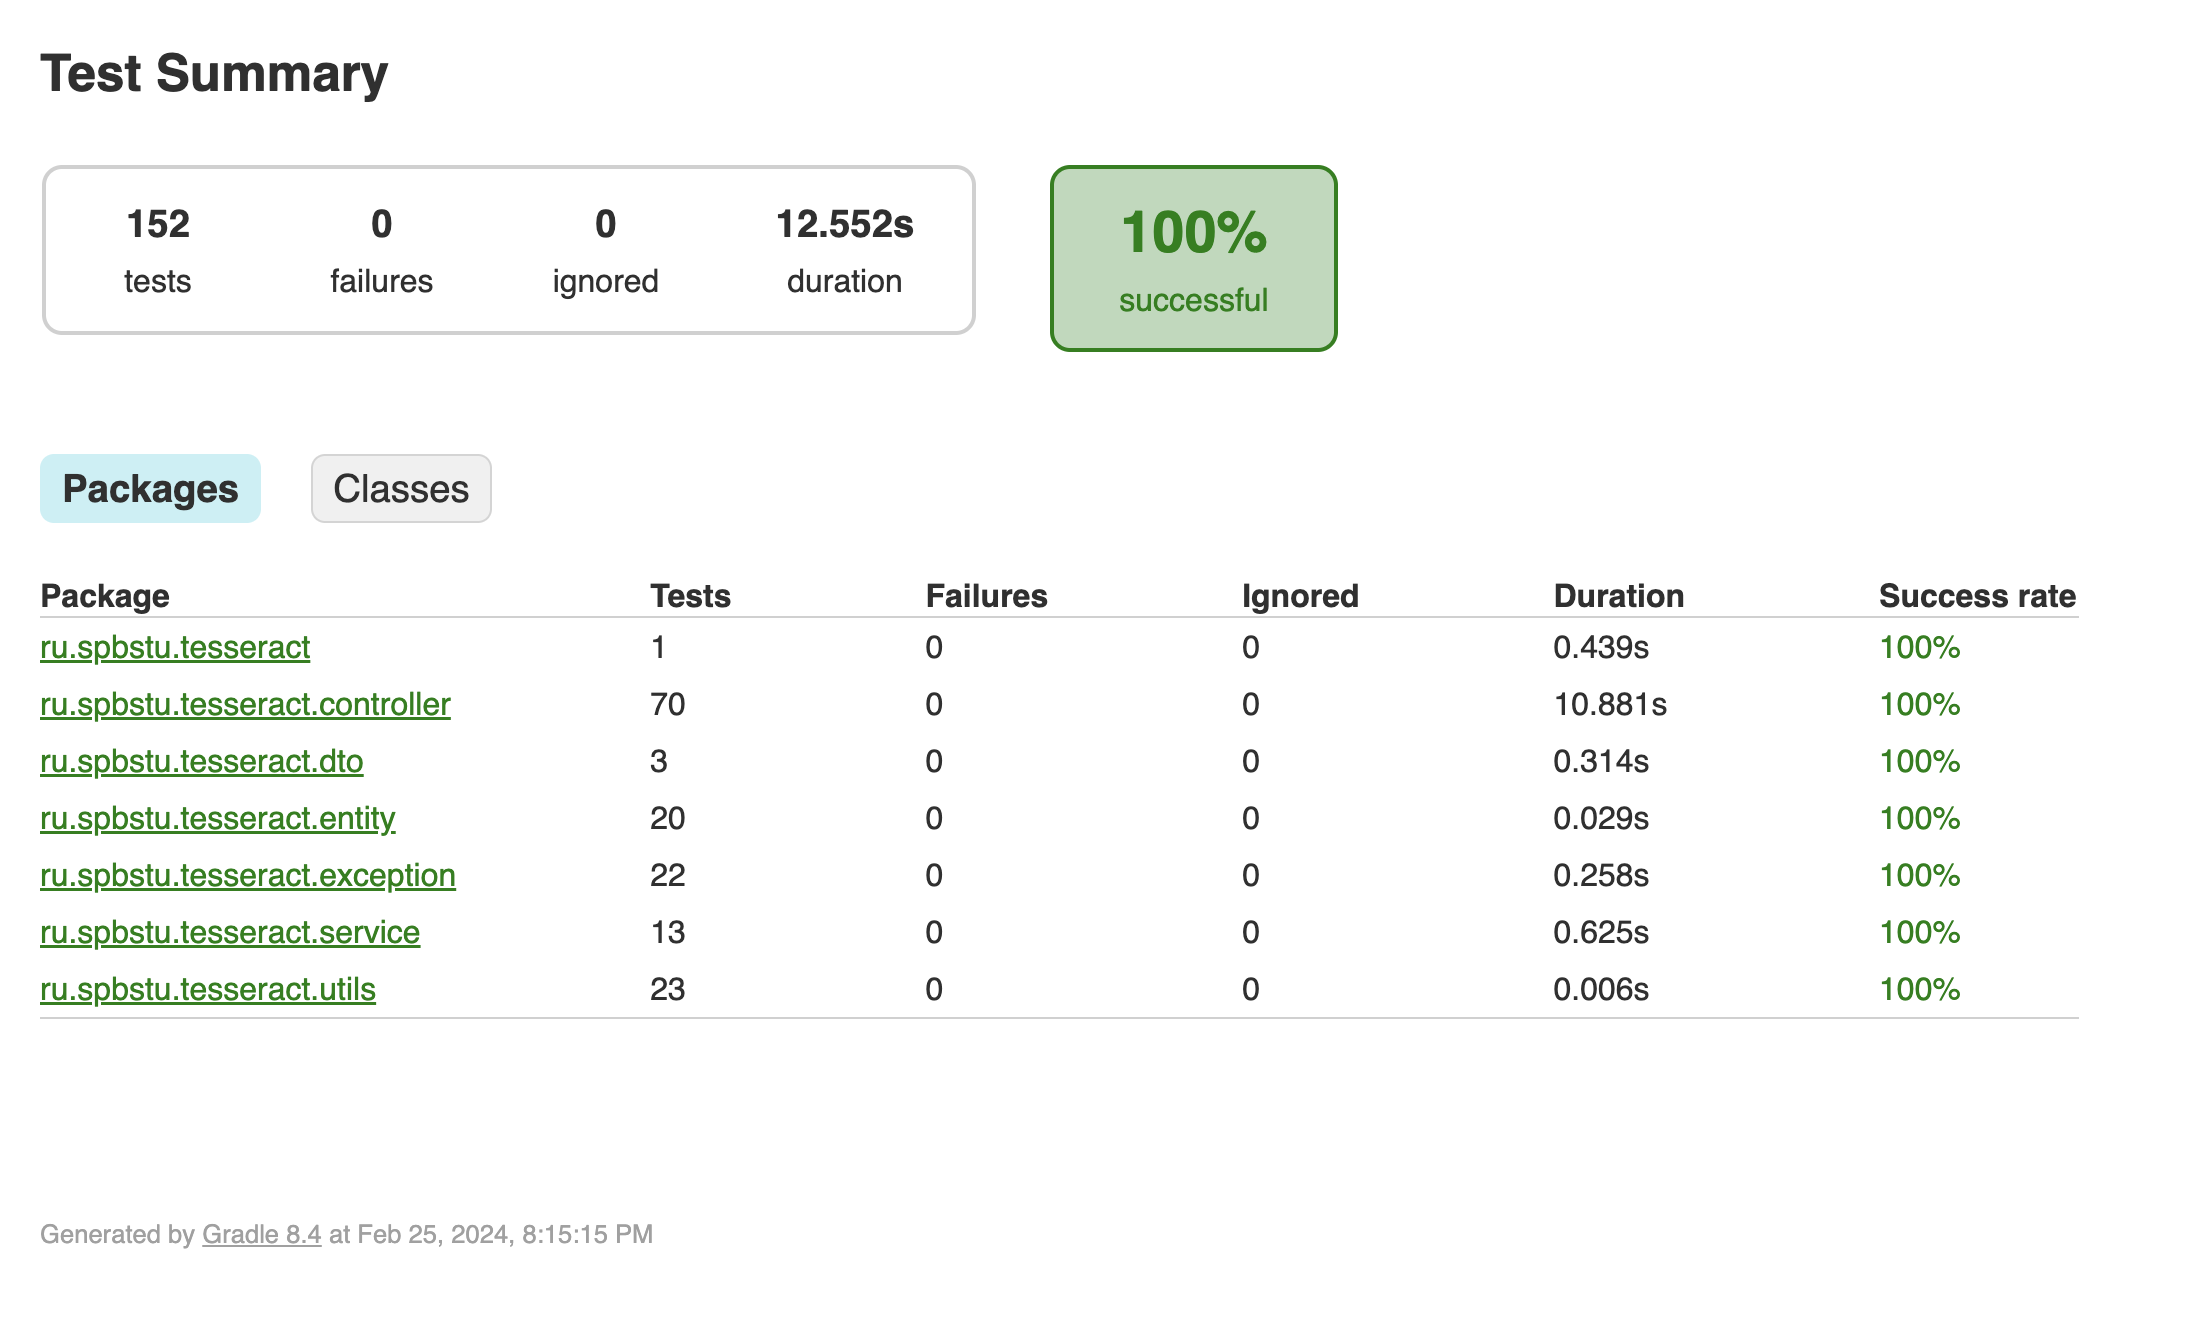
\includegraphics[width=15cm]{resources/3.png}\\
    \caption{Отчет о пройденных тестах}
\end{figure}

\subsection{Описание процедуры расширения тестового набора на примере добавления новой функциональной части (или модуля)}

При добавлении нового контроллера или же новых ручек для старого контроллера - их тестирование происходит по аналогии с уже существующими тестами.

\end{document}